\chapter{Theoretical Background on MIR and MER}
\label{chap:TheoreticalBackgroundMIRMER}
\thispagestyle{plain}

\vspace{0.5cm}

\noindent This chapter introduces the readers to the main basics about Music Information Retrieval and Music Emotion Recognition.

\section{Music Infomation Retrieval}
Music information retrieval (MIR) is the interdisciplinary science of retrieving information from music. MIR is a small but growing field of research with many real-world applications. Those involved in MIR may have a background in musicology, psychoacoustics, psychology, academic music study, signal processing, informatics, machine learning, optical music recognition, computational intelligence or some combination of these.
\\ \indent
MIR is being used by businesses and academics to categorize, manipulate and even create music.
\\
A few application to MIR can be:
\begin{itemize}
	\item Recommender systems: several already exixst, but few are based upon MIR techniques, instead making use of similarity between users or laborius data complilation as in \href{https://www.pandora.com}{Pandora}\footnote{https://www.pandora.com}.
	\item Intelligent and adaptive digital audio effects: aim of design a system that determine the settings of audio effects based on the audio content.
	\item Track separation and instrument recognition: like extracting the original tracks as recorded, which could have more than one instrument played per track. Instrument recognition is about identifying the instruments involved into one track.
	\item Automatic music transcription: process of converting na audio recording into symbolic, such score or a MIDI file.
	\item Automatic categorization: common task of MIR is musical genre categorization and is the usual task for the yearly Music Information Retrieval Evauation eXchange (MIREX).
\end{itemize}

\section{Music Emotion Recognition}
Music Emotion Recognition (MER) aim to research on modeling humans emotion perception of music \cite{yang2011music}, a research topic that emerges in the face of the explosice growth of digital music.
Automatic MER allows users to retrive and organiza their music collections in a fashion that is more content-centric than conventional metadata-based methods.
\\
The main challenge is based on the human perception of emotions, their subjective nature of emotion perception. 
Building such a music emotion recognition system, however, is challenging be- cause of the subjective nature of emotion perception. One needs to deal with issues such as the reliability of ground truth data and the difficulty in evaluating the prediction result, which do not exist in other pattern recognition problems such as face recognition and speech recognition. 
\\
MER methods developed try to address the issues related to the ambiguity and granularity of emotion description, the heavy cognitive load of emotion annotation, subjectivity of emotion perception, and the semantic gap between low-level audio signal and high-level emotion perception.

\subsection{Importance of Music Emotion Recognition}
Music plays an important role in human life, even more in the digital age. Never before has such a large collection of music been created and accessed daily by people. Before with the use of compact audio formats with near CD quality such as MP3 and now on with the various streaming services, have greatly contributed to the trmendous growth of digital music libraries.
\\ \indent
Conventionally, the management of music collections is based on catalog metadata, such as artist name, album name, and song title. As the amount of content continues to explode, this conventional approach may be no longer sufficient. The way that music information is organized and retrieved has to evolve to meet the ever increasing demand for easy and effective information access.
\\ \indent
Music, is a complex acoustic and temporal structure, it is rich in content and expressivity. When an individual engages with music as a composer, performer or listener, a very board range of mental processes is involved, including \textit{representational} and \textit{evaluative}. The representational process includes the perception of meter, rhythm, tonality, harmony, melody, form, and style, whereas the evaluative process includes the perception of preference, aesthetic experience, mood, and emotion. The term evaluative is used because such processes are typically both valenced and subjective. Both the representational and the evaluative processes of music listening can be leveraged to enhance music retrieval.
According to a study of \href{https://www.last.fm/home}{Last.fm}\footnote{https://www.last.fm/home}, emotion tagging is the third most frequent type of tags (first is genre and second locale) assigned to music pieces by online users.
\\ Even if emotion-based music retrieval was a new idea, a survey conducted in 2004 from \cite{lee2004survey} showed that about 28.2\% of the participants identified emotion as an important criterion in music seeking and organization.
\\ The table \ref{table:browse_music} represent the responses of 427 subjects to the question \textit{"When you search for music or music informations, how likely are you to use the following search/browse options?"} \cite{lee2004survey}.
\begin{table}[h!]
\centering
\begin{tabular}{|l | c|}
\hline
Search/Browse by & Positive rate\\ [0.5ex] 
\hline\hline Singer/Performer 			&		96.2\%	\\ 
\hline	Title of work(s) 					& 		91.6\%	\\ 
\hline	Some wors of the lyrics 	& 		74.0\% 	\\
\hline	Music style/genre 				&		62.7\%	\\
\hline	Reccomendations 				&		62.2\%	\\
\hline	Similar artist(s)					&		59.3\%	\\
\hline	Similar music 					&		54.2\%	\\
\hline	Associated usage				&		41.9\% 	\\
\hline	Singing								&		34.8\% 	\\
\hline	Theme(main subject)			&		33.4\% 	\\
\hline	Popularity							&		31.0\% 	\\
\hline	\textbf{Mood/emotional state	}	&		\textbf{28.2\%} 	\\
\hline	Time period						&		23.8\% 	\\
\hline	Occasions to use				&		23.6\% 	\\
\hline	Instrument(s)					&		20.8\% 	\\
\hline	Place/event where heard	&		20.7\% 	\\
\hline	Stroryline of music			&		17.9\% 	\\
\hline	Tempo								&		14.2\% 	\\
\hline	Record label						&		11.7\% 	\\
\hline	Publisher							&		6.0\% 	\\
\hline
\end{tabular}
\caption{Responses of 427 subjects to the question \textit{"When you search for music or music informations, how likely are you to use the following search/browse options?"}}
\label{table:browse_music}
\end{table}

Into another survey \cite{juslin2004expression}, they present findings from an exploratory questionnaire study featuring 141 music listeners (between 17 and 74 years of age) that offers some novel insights.
\\ 
One of the most exciting but difficult endeavors in research on music is to understand how listeners respond to music. It has often been suggested that a great deal of the attraction of music comes from its “emotional powers”. That is, people tend to value music because it expresses and induces emotions.
The table  \ref{table:motivation_music} tries to resume the motivations to the answer \textit{"Why do we listen to music?"}
\begin{table}[h!]
\centering
\begin{tabular}{|l | c|}
\hline
Motive & Ratio\\ [0.5ex] 
\hline\hline "To express, release and influence emotions"	&	47\%	\\ 
\hline "To relax and settle down"										&	33\%	\\
\hline "For enjoyment, fun, and pleasure"							&	22\%	\\
\hline "As company and background sound"						&	16\%	\\
\hline "Because it makes me feel good"								&	13\%	\\
\hline "Because it's a basic need, I can't live without it"		&	12\%	\\
\hline "Because I like, love music"										&	11\%	\\
\hline "To get energized"													&	9\%	\\
\hline "To evoke memories"												&	4\%	\\ 
\hline
\end{tabular}
\caption{Responses of 141 subjects to the question \textit{"Why do you listen to music?"}}
\label{table:motivation_music}
\end{table}

\indent
Some music companies, like  \href{https://www.allmusic.com/moods}{Allmusic.com}\footnote{https://www.allmusic.com/moods}, gives the possibility to search music by emotion labels. With these, the user can retrive and browse artists or albums by emotion.
\\ \indent
Making computers capable of recognizing the emotion of music also enhances the way humans and computers interact. It is possible to play back music that matches the user’s mood detected from physiological, prosodic, or facial cues. A cellular phone equipped with automatic music emotion recognition (MER) function can then play a song best suited to the emotional state of the user; a smart space (e.g., restaurant, conference room, residence) can play background music best suited the people inside it.

\subsection{Recognizing the perceived emotion of music}
There is a relationship between music and emotions, that has been the subject of much discussion and research in many different disciplines, like philosphy, musicology, sociology.
\\
In psychological studies, emotion are often divided into three categories:
\begin{itemize}
	\item \textit{Expressed emotion}: the ones the performer tries to communicate with the listener.
	\item \textit{\textbf{Perceived emotion}}: represented by music and perceived by the listener.
	\item \textit{Felt or Evoked emotion}: induced by music and felt by the listener.
\end{itemize}

MER focus on perceived emotions because they are less subjective than felt emotions and are often easier to conceptualize. This because felt emotions depends on personal factors and the situation in which the listener processes the song.
From an engineering point of view, one of the main interests is to develpo a computational model of music emotion and to facilitate emotion-based music retrieval and organization. MIR community has made many efforts for automatic recogition of the perceived emotion of music, various implementations will be presented further in chapter \ref{chap:StateOfTheArt}.
\\
A typical approach to MER categorizes emotions into a number of classes and applies Machine Learning (ML) techniques to train a classifies. Usually are extracted some features of music to represent the acoustic property of a music piece. Typically, a subjective test is conducted to collect the ground truth needed for training the computational model of emotion prediction. Subjects are asked to report their emotion perceptions of the music pieces.
\\
To learn the relationship between music features and emotion labels have been applied, such as Support Vector Machines (SVMs), Gaussian Mixture Models (GMMs), Neural Networks (NN) and k-nearest neighbor.
\\
After training, the automatic model can be applied to classify the emotion of an input music piece, for example a schematic diagram of the \textit{cathegorical approach} to MER can be seen in figure \ref{fig:MER_categorical_approach}.

\begin{figure}[h]
    \centering
    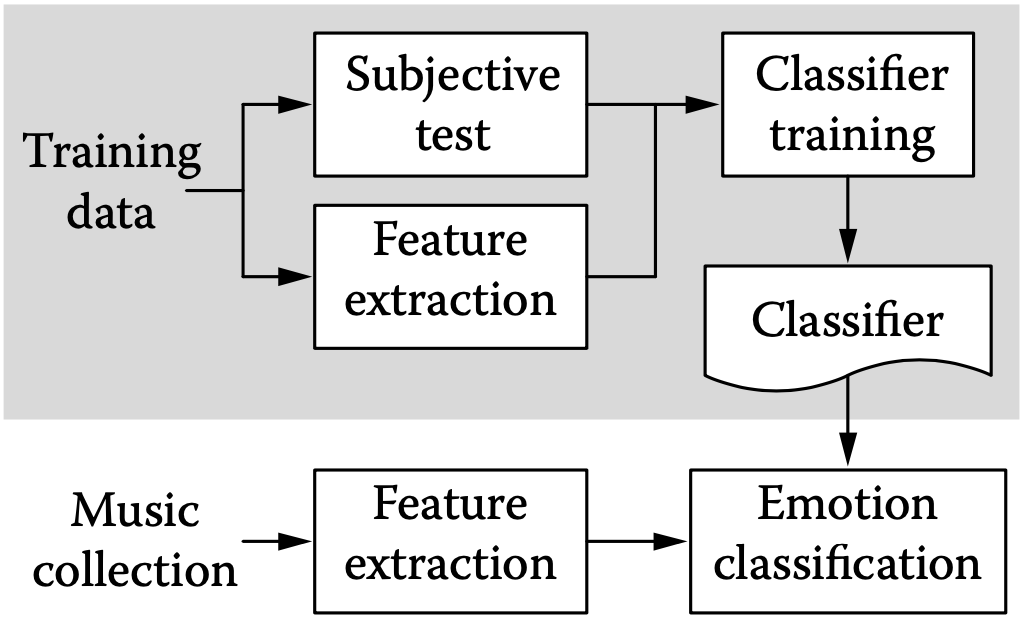
\includegraphics[scale=0.5]{MER_categorical_approach.png} 
	\caption{Schematic diagram of the categorical approach to MER}
    \label{fig:MER_categorical_approach}
\end{figure}

\subsection{Open issues of Music Emotion Recognition}
As MER is a quite new domain, there are some elements that have no clear answer. Four of these issues are:
\begin{enumerate}
	\item Ambiguity and Granularity of emotion description:
	\item Heavy cognitive load of emotion annotation
	\item Subjectivity of emotional perception:
	\item Semantic gap between Low-Level (LL) and audio signal and High Level (HL) Human perception:
\end{enumerate}





